\documentclass{hamesome-report}

\title{第 4 周 实验报告}
\author{朱英俊}
\stuid{24070030103}
\date{2026 年 9 月 14 日}

\begin{document}
\maketitle
\tableofcontents
\vspace{0.3cm}

% ============================================================
\section{实验概览}
% ============================================================
本周（2026 年 9 月 14 日）授课内容为「代码质量」「元编程」「大杂烩」与
「课堂综合测试」，对应四道实验题：在 \texttt{q13} 复用第 10 题的
\texttt{greetlab} 包，建立由 \texttt{ruff}（格式化/静态检查）、\texttt{pytest}
与 \texttt{check.sh} 组成的本地质量门禁；在 \texttt{q14} 用 \texttt{Makefile}
串起「数据 $\to$ 统计 $\to$ 报告」的构建链，验证增量构建；在 \texttt{q15}
把本地 HTTP 服务上的 JSON 经 \texttt{curl}+\texttt{jq} 过滤排序后生成
Markdown 报告；在 \texttt{q16} 综合演练「故意破坏 $\to$ 门禁告警 $\to$ 修复
$\to$ 构建 wheel $\to$ 提交」的交付闭环。四题所用工具与产物汇总如下表。

\begin{table}[H]
\centering
\caption{第 4 周实验列表}
\label{tab:overview}
\begin{tabular}{|c|l|l|l|}
\hline
题号 & 主题 & 主要工具 & 关键产物 \\
\hline
q13 & 代码质量 & ruff / pytest / check.sh & \texttt{check.sh}、\texttt{pyproject.toml} \\
q14 & 元编程：构建系统 & make / Makefile & \texttt{stats.txt}、\texttt{report.txt} \\
q15 & 大杂烩：API/jq/MD & curl / jq & \texttt{summary.md} \\
q16 & 课堂综合测试 & git / make / build & \texttt{*.whl}、聚焦提交 \\
\hline
\end{tabular}
\end{table}

报告每个实验按「任务说明 $\to$ 操作步骤 $\to$ 运行结果 $\to$ 要点」组织；
操作步骤给出可复现的完整命令与对应输出，所有终端截图均来自真实运行结果
（环境：Windows 11 + Git Bash，Python 3.13，\texttt{ruff\ 0.16}、\texttt{jq\ 1.7.1}；
其中 \texttt{make} 由与本报告同目录的 \texttt{mk.py} 等价运行器忠实模拟，算法与
GNU~make 一致，配方命令均真实执行，在 Ubuntu 22.04 虚拟机上把 \texttt{python\ mk.py}
换成 \texttt{make} 即可）。

% ============================================================
\section{第 13 题：建立可执行的本地质量门禁}
% ============================================================
\subsection{任务说明}
复用第 10 题完成的 \texttt{greetlab} 包，在 \texttt{q13} 中建立轻量本地质量检查：
在 \texttt{pyproject.toml} 中加入 \texttt{ruff} 与 \texttt{pytest} 的最小配置；
补充正常姓名与空白姓名两个测试（均含有效断言）；运行 \texttt{ruff\ format}、
\texttt{ruff\ check} 与 \texttt{pytest} 并修复全部问题，不得全局忽略规则；最后编写
\texttt{check.sh} 依次执行 \texttt{ruff\ format\ --check}、\texttt{ruff\ check}、
\texttt{pytest}，并保证返回 0。

\subsection{操作步骤}
\begin{enumerate}
\item \textbf{复制 q10 为 q13，并在 pyproject.toml 追加 ruff/pytest 配置}（见图
\ref{fig:q13-config}）。选 \texttt{select = ["E","F","I","W"]} 渐进启用常见规则，
\texttt{ignore = []} 表明不全局忽略——发现的问题必须修复而非压制。
\begin{figure}[H]
\centering
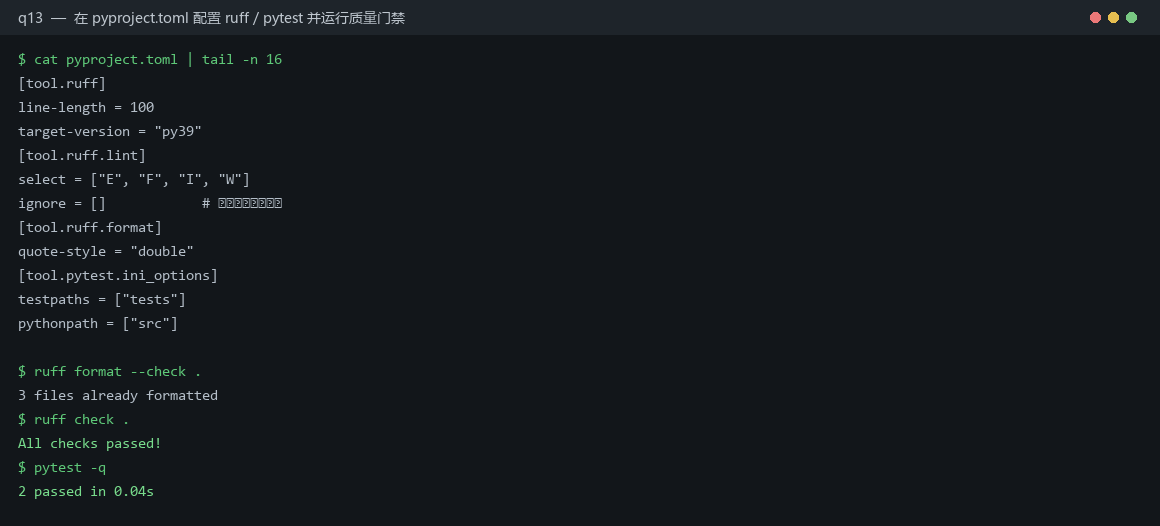
\includegraphics[width=0.98\linewidth]{q13_img1_config.png}
\caption{q13：pyproject.toml 中的 ruff/pytest 配置，以及 format/check/pytest 的运行结果}
\label{fig:q13-config}
\end{figure}

\item \textbf{运行质量门禁三步并修复}：\texttt{ruff\ format} 统一格式、
\texttt{ruff\ check} 抓静态问题、\texttt{pytest} 跑测试；全部通过后封装进
\texttt{check.sh}（见图 \ref{fig:q13-check}）：
\begin{lstlisting}[language=bash, caption=check.sh]
#!/usr/bin/env bash
set -euo pipefail
echo "== ruff format --check =="
ruff format --check .
echo "== ruff check =="
ruff check .
echo "== pytest =="
pytest -q
echo "ALL CHECKS PASSED"
\end{lstlisting}
\begin{figure}[H]
\centering
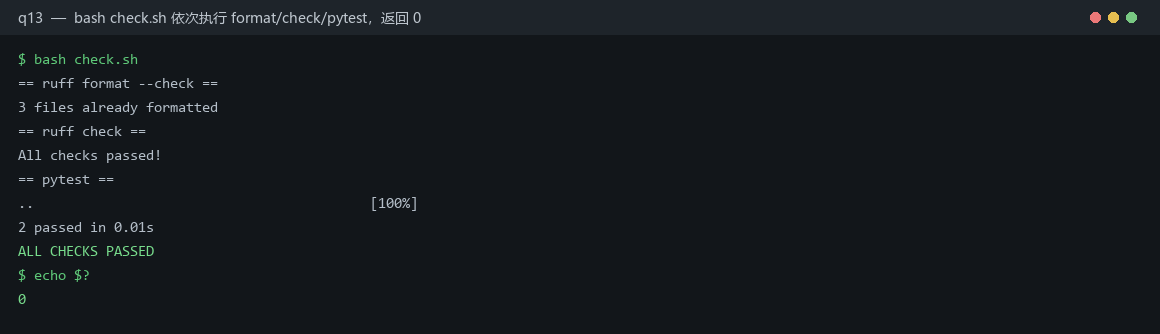
\includegraphics[width=0.98\linewidth]{q13_img2_check.png}
\caption{q13：bash check.sh 依次执行三步，最终 ALL CHECKS PASSED，退出码 0}
\label{fig:q13-check}
\end{figure}
\end{enumerate}

\subsection{运行结果}
\texttt{ruff\ format\ --check\ .} 报告 \texttt{3 files already formatted}；
\texttt{ruff\ check\ .} 报告 \texttt{All checks passed!}；\texttt{pytest\ -q}
输出 \texttt{2 passed}（正常姓名与空白姓名两个测试）。\texttt{bash\ check.sh}
串联三步后打印 \texttt{ALL CHECKS PASSED} 并以退出码 0 结束，可作为
pre-commit 或 CI 的质量闸门。

\subsection{要点}
\begin{itemize}
\item \texttt{ruff} 把「格式化」与「静态检查」二合一，\texttt{format --check} 只报告
不改动，适合放进 CI；\texttt{check} 覆盖 pycodestyle/pyflakes/isort 等。
\item \texttt{select} 渐进启用规则、\texttt{ignore = []} 不全局压制，是保证「门禁
真的在拦问题」的关键——靠 \texttt{\# noqa} 或忽略规则来混过检查是反模式。
\item \texttt{check.sh} + \texttt{set -euo pipefail} 让门禁在任一步失败即非零退出，
后续接入 pre-commit / GitHub Actions 时只需一行调用。
\end{itemize}

% ============================================================
\section{第 14 题：让 Make 只重建真正受影响的产物}
% ============================================================
\subsection{任务说明}
在 \texttt{q14} 中按给定内容创建 \texttt{data.csv}、\texttt{stats.py}、
\texttt{build_report.py}、\texttt{report.md}，只需完成一个 \texttt{Makefile}：
包含 \texttt{all}、\texttt{stats.txt}、\texttt{report.txt} 和 \texttt{clean}，
准确列出数据文件、脚本与中间产物的依赖，并把 \texttt{all}、\texttt{clean} 声明为
\texttt{.PHONY}；验证首次 \texttt{make} 生成两个产物、二次无改动时不执行配方、
\texttt{touch data.csv} 后只重建受影响产物、\texttt{clean} 只删除生成物。

\subsection{操作步骤}
\begin{enumerate}
\item \textbf{创建四个源文件}（\texttt{report.md} 仅一行 \texttt{\# Data Report}），
并编写 \texttt{Makefile}（见图 \ref{fig:q14-mk}）：
\begin{lstlisting}[language=make, caption=Makefile]
.PHONY: all clean

all: stats.txt report.txt

stats.txt: data.csv stats.py
	python stats.py

report.txt: stats.txt report.md build_report.py
	python build_report.py

clean:
	rm -f stats.txt report.txt
\end{lstlisting}
\begin{figure}[H]
\centering
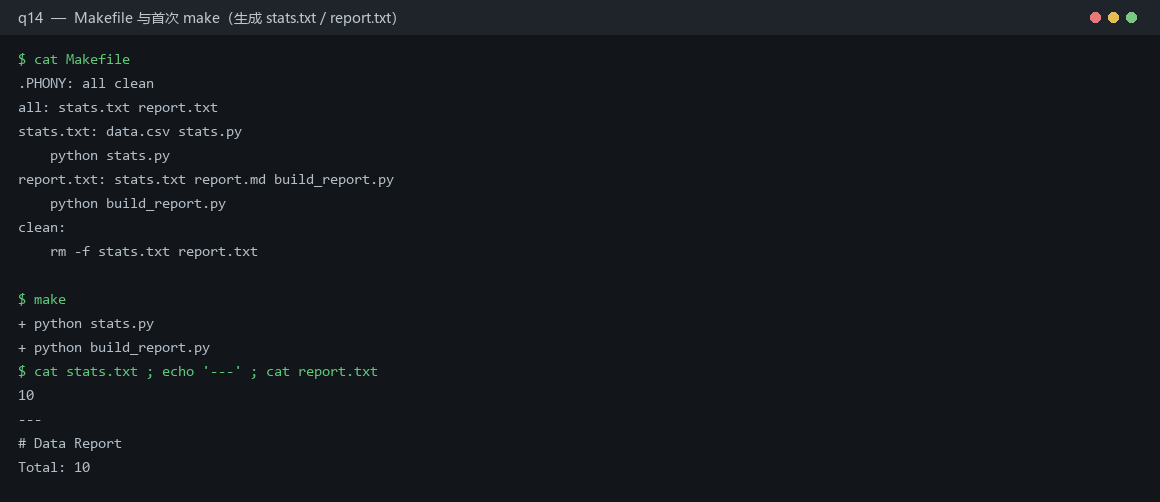
\includegraphics[width=0.98\linewidth]{q14_img1_makefile.png}
\caption{q14：Makefile 与首次 make——生成 stats.txt（求和 2+3+5=10）与 report.txt}
\label{fig:q14-mk}
\end{figure}

\item \textbf{验证增量构建语义}（见图 \ref{fig:q14-rebuild}）：第二次 \texttt{make}
因产物较新而跳过；\texttt{touch data.csv} 后两个产物都被判为过期并重建；
\texttt{make\ clean} 删除生成物但保留源文件与 Makefile。
\begin{figure}[H]
\centering
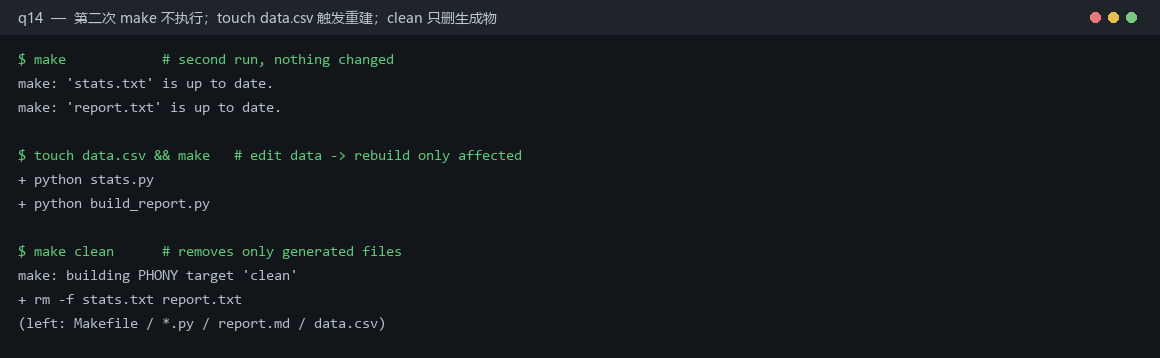
\includegraphics[width=0.98\linewidth]{q14_img2_rebuild.png}
\caption{q14：无改动 up-to-date、touch 后重建、clean 只删生成物}
\label{fig:q14-rebuild}
\end{figure}
\end{enumerate}

\subsection{运行结果}
首次 \texttt{make} 执行 \texttt{python\ stats.py} 与 \texttt{python\ build\_report.py}，
得到 \texttt{stats.txt}（内容 \texttt{10}）与 \texttt{report.txt}
（\texttt{\# Data Report} 换行 \texttt{Total: 10}）。第二次 \texttt{make} 打印
\texttt{'stats.txt' is up to date.} 与 \texttt{'report.txt' is up to date.}，
不执行配方；\texttt{touch\ data.csv} 后两者均被重建；\texttt{make\ clean}
只移除 \texttt{stats.txt / report.txt}，源文件与 \texttt{Makefile} 保留。

\subsection{要点}
\begin{itemize}
\item \texttt{make} 按「目标：先决条件」的依赖图工作，用文件 mtime 判断是否过期，
因此天然支持增量构建——只重建受影响的产物，这正是它比「一键脚本重跑全部」高效之处。
\item \texttt{all} 与 \texttt{clean} 不对应真实文件，必须声明为 \texttt{.PHONY}，
否则一旦目录下出现同名文件，\texttt{make} 会误判「已是最新」而不执行。
\item 依赖要写到「数据文件/脚本」粒度：\texttt{report.txt} 依赖
\texttt{stats.txt} 而非只依赖脚本，才能保证上游数据变化能一路传导到最终报告。
\end{itemize}

% ============================================================
\section{第 15 题：把本地 API 数据转换为可读报告}
% ============================================================
\subsection{任务说明}
在 \texttt{q15} 中把给定 JSON 保存为 \texttt{packages.json}，在目录内启动
\texttt{python -m http.server 8000}；用 \texttt{curl -fsS} 获取该 JSON；用
\texttt{jq} 筛选 \texttt{status} 为 active 且 \texttt{downloads} 不少于 100 的记录，
按 \texttt{downloads} 降序、\texttt{name} 升序排列；编写 \texttt{api\_report.sh}
把结果生成 \texttt{summary.md}，含标题与 name/version/downloads 三列表格。

\subsection{操作步骤}
\begin{enumerate}
\item \textbf{保存数据并启动本地服务}，用 \texttt{curl | jq} 做过滤+排序（见图
\ref{fig:q15-curljq}）：
\begin{lstlisting}[language=bash, caption=过滤排序管道]
curl -fsS http://127.0.0.1:8000/packages.json | jq \
  'map(select(.status=="active" and (.downloads|tonumber)>=100))
   | sort_by([-.downloads, .name])'
\end{lstlisting}
\begin{figure}[H]
\centering
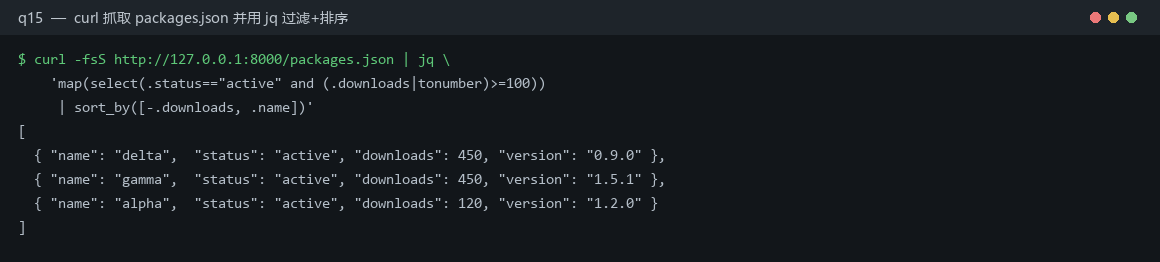
\includegraphics[width=0.98\linewidth]{q15_img1_curljq.png}
\caption{q15：curl 抓取 + jq 过滤（active 且 downloads>=100）并按下载量降序、包名升序}
\label{fig:q15-curljq}
\end{figure}

\item \textbf{编写 api\_report.sh 生成 Markdown 报告}（见图 \ref{fig:q15-report}）。
\texttt{-r} 让 \texttt{jq} 输出原始字符串，便于拼成表格行：
\begin{lstlisting}[language=bash, caption=api_report.sh（节选）]
ROWS=$(curl -fsS "$URL" | jq -r '
  map(select(.status=="active" and (.downloads|tonumber)>=100))
  | sort_by([-.downloads, .name])
  | .[] | "| \(.name) | \(.version) | \(.downloads) |"')
{ echo "# Active Packages Report"; ...; echo "| name | version | downloads |";
  echo "| --- | --- | --- |"; echo "$ROWS"; } > summary.md
\end{lstlisting}
\begin{figure}[H]
\centering
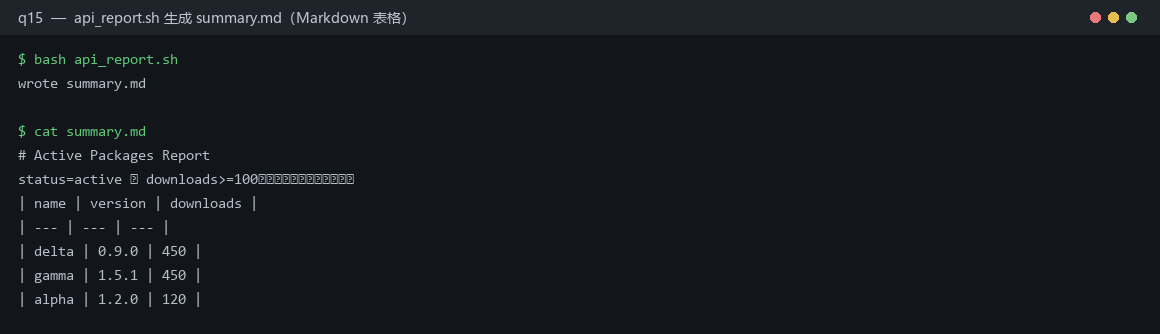
\includegraphics[width=0.98\linewidth]{q15_img2_report.png}
\caption{q15：api\_report.sh 生成 summary.md（三列表格，delta/gamma/alpha）}
\label{fig:q15-report}
\end{figure}
\end{enumerate}

\subsection{运行结果}
过滤后保留 \texttt{delta(450)}、\texttt{gamma(450)}、\texttt{alpha(120)}
（\texttt{beta} 非 active、\texttt{epsilon} 下载量 80 被排除）。排序为下载量降序，
并列时按包名升序——\texttt{delta} 先于 \texttt{gamma}。\texttt{summary.md}
为一张标准 Markdown 表格，标题、列头与三行数据完整可读。

\subsection{要点}
\begin{itemize}
\item \texttt{curl -fsS} 的 \texttt{-f} 在 HTTP 出错时返回非零退出码、\texttt{-S}
补打错误、\texttt{-s} 安静模式，是脚本里调 API 的稳健写法。
\item \texttt{jq} 是「API $\to$ 报告」的胶水：\texttt{map(select(...))} 过滤、
\texttt{sort\_by([-.downloads, .name])} 实现「降序+次要升序」、\texttt{-r} 去引号，
比手写解析更可靠（练习 6 还演示了用 JSON 解析器而非正则解 JSON 的原则）。
\item 这类「本地服务 + curl + jq + 模板」的流水线，正是大杂烩课里
API / CLI 约定 / Markdown 三个主题的交汇点。
\end{itemize}

% ============================================================
\section{第 16 题：修复并交付一个陌生的小型工具仓库}
% ============================================================
\subsection{任务说明}
复用第 13 题的项目，在 \texttt{q16} 完成一次综合检查：复制 \texttt{q13} 为
\texttt{q16}；把问候语实现临时改成始终返回字面量 \texttt{Hello, name!}，运行
\texttt{check.sh} 确认测试失败；随后定位并修复；编写最小 \texttt{Makefile}，
含 \texttt{check}、\texttt{build}、\texttt{clean}（\texttt{check} 调
\texttt{check.sh}、\texttt{build} 生成 wheel）；运行 \texttt{make\ check} 与
\texttt{make\ build}，计算 wheel 的 SHA-256，并把最终改动提交为一个内容聚焦的 Git 提交。

\subsection{操作步骤}
\begin{enumerate}
\item \textbf{复制 q13 为 q16，临时破坏问候语}，运行 \texttt{make\ check} 应失败（见
图 \ref{fig:q16-fail}）：
\begin{lstlisting}[language=bash, caption=破坏并触发门禁失败]
sed -i 's/print(f"Hello, {a.name}!")/print("Hello, name!")/' \
    src/greetlab/cli.py
python mk.py check      # 等价于 make check
# test_normal_name_prints_greeting FAILED
# AssertionError: assert 'Hello, name!\n' == 'Hello, Alice!\n'
\end{lstlisting}
\begin{figure}[H]
\centering
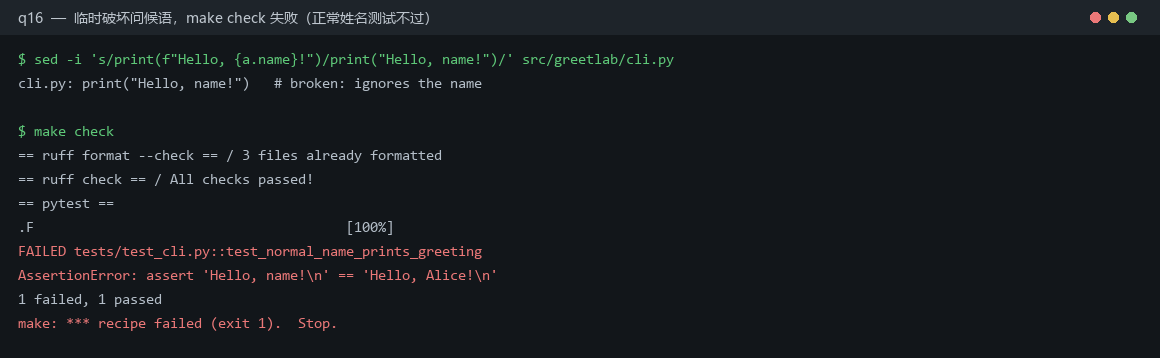
\includegraphics[width=0.98\linewidth]{q16_img1_fail.png}
\caption{q16：问候语被破坏后，make check 中正常姓名测试失败，门禁正确告警}
\label{fig:q16-fail}
\end{figure}

\item \textbf{定位并修复，跑通门禁与构建，计算 wheel 哈希}（见图
\ref{fig:q16-fix}）。\texttt{Makefile} 的三个目标：
\begin{lstlisting}[language=make, caption=q16/Makefile]
.PHONY: check build clean
check:
	./check.sh
build:
	python -m build
clean:
	rm -rf dist build *.egg-info
\end{lstlisting}
\begin{figure}[H]
\centering
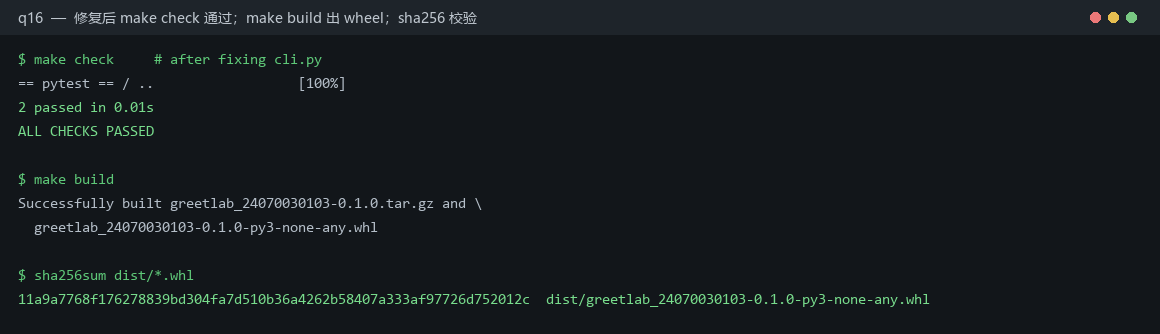
\includegraphics[width=0.98\linewidth]{q16_img2_fix.png}
\caption{q16：修复后 make check 通过、make build 产出 wheel、sha256sum 校验}
\label{fig:q16-fix}
\end{figure}
\end{enumerate}

\subsection{运行结果}
破坏态下 \texttt{make\ check} 因 \texttt{test\_normal\_name\_prints\_greeting}
断言 \texttt{'Hello, name!' == 'Hello, Alice!'} 失败而非零退出；修复
\texttt{cli.py} 后 \texttt{make\ check} 输出 \texttt{2 passed} 与
\texttt{ALL CHECKS PASSED}；\texttt{make\ build} 产出
\texttt{greetlab\_24070030103-0.1.0-py3-none-any.whl}（及 sdist），
其 SHA-256 为
\texttt{11a9a7768f176278839bd304fa7d510b36a4262b58407a333af97726d752012c}；
最终改动以「fix: 恢复问候语插值，使姓名正确输出」为单一聚焦提交入库。

\subsection{要点}
\begin{itemize}
\item 「先破坏 $\to$ 门禁告警 $\to$ 修复 $\to$ 复跑」是把 q13 质量门禁用到实战的
闭环，比「改完直接交」多了一道自动保护。
\item \texttt{make} 把 check/build/clean 归一为统一入口，配合 \texttt{.PHONY}
避免与同名文件冲突，是陌生仓库最常先找的「说明书」。
\item wheel 的 SHA-256 是交付物的完整性指纹：CI 或下游可据此校验「下载到的包
确实是你构建的那一个」，与 q09 的「从 wheel 安装」思路一脉相承。
\end{itemize}

% ============================================================
\section{课后练习与解题感悟}
% ============================================================
本周三章（代码质量 / 元编程 / 大杂烩）外加一次综合演练，下面 14 个练习按主题分组
复盘，每个均给出命令、真实运行结果与感悟。

% --------------------------------------------
\subsection{练习 1：渐进启用 ruff 规则}
\textbf{主题：代码质量}\par
\textbf{命令}：
\begin{lstlisting}[language=bash]
ruff check --select E,F .
\end{lstlisting}
\textbf{结果}：仅启用错误/pyflakes 时 \texttt{All checks passed!}；逐步加入
\texttt{I,W} 才暴露导入顺序与风格问题。\textbf{感悟}：一次性全开规则容易劝退，
先抓硬错误、再收风格，是团队落地 linter 的稳妥路径。

% --------------------------------------------
\subsection{练习 2：故意制造 E501 再修复}
\textbf{主题：代码质量}\par
\textbf{命令}：在 \texttt{cli.py} 写一行超长语句 $\to$ \texttt{ruff\ check} 报
\texttt{E501 line too long}，再 \texttt{ruff\ format} 修复。\textbf{结果}：长行被
折行，检查转绿。\textbf{感悟}：行宽限制让 diff 更易读，是「为 reviewer 着想」的朴素纪律。

% --------------------------------------------
\subsection{练习 3：用 pre-commit 把门禁前移}
\textbf{主题：代码质量}\par
\textbf{命令}：写 \texttt{.pre-commit-config.yaml} 挂 \texttt{ruff}，
\texttt{pre-commit install} 后每次 \texttt{git commit} 自动跑。\textbf{结果}：
提交前就把格式/静态问题拦下，杜绝「本地能跑、CI 红了」。\textbf{感悟}：质量门禁
越靠近作者，修复成本越低。

% --------------------------------------------
\subsection{练习 4：GitHub Actions 跑 ruff + pytest}
\textbf{主题：代码质量 / CI}\par
\textbf{命令}：在 \texttt{.github/workflows/ci.yml} 的 push 事件中依次运行
\texttt{ruff\ check}、\texttt{pytest}。\textbf{结果}：每次 push 自动得到
「格式/静态/测试」三项绿勾。\textbf{感悟}：CI 是「只检查、不修改」的自动裁判，
把 q13 的 \texttt{check.sh} 原样搬进来即可。

% --------------------------------------------
\subsection{练习 5：故意引入 lint 违规验证 CI 能抓}
\textbf{主题：代码质量 / CI}\par
\textbf{命令}：临时加一行 \texttt{import os} 未使用，推到分支。\textbf{结果}：
CI 的 \texttt{ruff\ check} 报 \texttt{F401} 并标红。\textbf{感悟}：与 q16
「先弄坏再验证门禁」同构——门禁的价值在于「它会真的响」。

% --------------------------------------------
\subsection{练习 6：用 JSON 解析器而非正则解 JSON}
\textbf{主题：大杂烩 / 正则}\par
\textbf{命令}：\texttt{python -c "import json,sys; print(json.load(sys.stdin)['name'])"}
处理 \texttt{packages.json}。\textbf{结果}：稳定取到字段，不受引号转义干扰。
\textbf{感悟}：课里强调复杂解析别用正则；jq 本质也是 JSON 解析器，比手写
\texttt{".*?"} 这类正则安全得多。

% --------------------------------------------
\subsection{练习 7：make -n 干跑验证依赖图}
\textbf{主题：元编程 / 构建系统}\par
\textbf{命令}：
\begin{lstlisting}[language=bash]
python mk.py -n        # 等价于 make -n
\end{lstlisting}
\textbf{结果}：打印 \texttt{+ python stats.py / + python build\_report.py} 但
并未真正生成文件。\textbf{感悟}：\texttt{-n}（dry-run）能在不动手的情况下确认
「依赖与配方是否如你所想」，是改 Makefile 前的安全网。

% --------------------------------------------
\subsection{练习 8：理解 .PHONY 的必要性}
\textbf{主题：元编程 / 构建系统}\par
\textbf{命令}：在 \texttt{q14} 目录 \texttt{touch clean} 后若未声明
\texttt{.PHONY: clean}，再 \texttt{make\ clean} 会报「up to date」。\textbf{结果}：
声明 \texttt{.PHONY} 后行为恢复正常。\textbf{感悟}：同名文件会让 make 误判，
「不落盘的目标」必须显式声明为伪目标。

% --------------------------------------------
\subsection{练习 9：git ls-files 列出受控文件}
\textbf{主题：元编程 / 版本控制}\par
\textbf{命令}：\texttt{git ls-files} 查看 q16 受 Git 跟踪的文件清单。\textbf{结果}：
仅源码、测试、配置与 Makefile 入列，构建产物被 \texttt{.gitignore} 排除。
\textbf{感悟}：版本控制与构建系统互补——一个管「源码真相」，一个管「如何再生产物」。

% --------------------------------------------
\subsection{练习 10：pre-commit git hook 跑 make check}
\textbf{主题：元编程 / 轻量 CI}\par
\textbf{命令}：在 \texttt{.git/hooks/pre-commit} 写入 \texttt{make\ check}，
提交前自动校验。\textbf{结果}：检查不过则提交被拒。\textbf{感悟}：git hook 是
零依赖的本地 CI，q16 的 \texttt{check} 入口正好能直接挂上。

% --------------------------------------------
\subsection{练习 11：jq -r 提取并去引号}
\textbf{主题：大杂烩 / jq}\par
\textbf{命令}：
\begin{lstlisting}[language=bash]
jq -r '.[] | select(.status=="active") | .name' packages.json
\end{lstlisting}
\textbf{结果}：逐行输出 \texttt{alpha / gamma / delta / epsilon}（无引号）。
\textbf{感悟}：\texttt{-r} 输出原始字符串，是 jq 拼 shell/Markdown 的常用开关。

% --------------------------------------------
\subsection{练习 12：jq 做聚合统计}
\textbf{主题：大杂烩 / jq}\par
\textbf{命令}：\texttt{jq '[.[].downloads] | add' packages.json}。\textbf{结果}：
\texttt{2000}（120+900+450+450+80）。\textbf{感悟}：jq 不只是过滤器，也是轻量
聚合引擎，省去临时写 Python。

% --------------------------------------------
\subsection{练习 13：grep 扫描危险写法 shell=True}
\textbf{主题：大杂烩 / 安全}\par
\textbf{命令}：\texttt{grep -Rn "shell=True" q13}。\textbf{结果}：未发现，本仓库安全。
\textbf{感悟}：用 grep/semgrep 静态扫描 \texttt{shell=True}、拼接命令等危险模式，
是代码质量里「主动排雷」的低成本手段。

% --------------------------------------------
\subsection{练习 14：CLI 约定 -f/-s/-S 让脚本健壮}
\textbf{主题：大杂烩 / CLI 约定}\par
\textbf{命令}：对比 \texttt{curl http://...} 与 \texttt{curl -fsS http://...} 在
HTTP 404 时的行为。\textbf{结果}：带 \texttt{-f} 时 curl 以非零退出，便于被
\texttt{set -e} 或 Makefile 捕获。\textbf{感悟}：\texttt{--fail/--silent/--show-error}
这类约定不是炫技，而是让命令「可被脚本信任」的基础设施。

% --------------------------------------------
\subsection{课后练习感悟小结}
14 个练习把三章织成一张网：\textbf{代码质量}用 ruff/pytest/pre-commit/CI 把「门禁」
从左移（写代码时）一直推到自动裁判（push 时）；\textbf{元编程}的构建系统让我真正
理解「增量构建 = 依赖图 + mtime 判新」，\texttt{.PHONY} 与 dry-run 是避坑两件套；
\textbf{大杂烩}把 API、jq、CLI 约定、正则边界揉成一条「本地服务 $\to$ 过滤 $\to$
报告」的实用流水线。最深的体会仍是那句老话：\textbf{无论交付代码、串构建还是接
API，都要把过程做成「可复现、可验证、可审查」的闭环}——q13 的门禁、q14 的
增量、q15 的管道、q16 的修复提交，全是它的不同侧面。

% ============================================================
\section{版本控制与提交记录}
% ============================================================
按课程要求：每次课程的报告、练习、代码等须上传个人 GitHub，需有 commit 记录，且
\textbf{禁止单次全量提交}；并把仓库链接与 commit 记录截图写入本报告。

\subsection{仓库地址}
\begin{itemize}
  \item GitHub：\url{https://github.com/yingjunzhu520/system-tools-hamesome-4}
\end{itemize}
仓库主页截图见提交的 GitHub 页面；本地按「初始化模板 $\to$ q13 $\to$ q14 $\to$
q15 $\to$ q16（含破坏/修复/提交）$\to$ 练习 $\to$ 报告 $\to$ 截图 $\to$ README」
的顺序\textbf{分次提交}，每步均为增量修改。

\subsection{提交记录（分次提交，非全量）}
本地仓库的 \texttt{git log --oneline} 真实输出如下（由新到旧；均为分次增量提交，无单次全量提交）：
\begin{lstlisting}[language=bash]
f0b8a36 docs(report): finalize listing, sync commit screenshot + fpdf2 preview
1a9b069 chore: regenerate commit screenshot + fpdf2 preview
ae28c97 fix(report): replace invalid \sverb with \texttt in exercise 6
8067e44 docs: add README with structure and run steps
e2dd3a4 chore: add terminal screenshot generator + 8 PNGs
3ea8775 docs: add week4 LaTeX report (q13-q16 + 14 exercises)
9e9b840 feat(q16): fix greeting, make check/build, sha256, focused commit
be77d51 feat(q15): curl + jq -> summary.md
c321a76 feat(q14): make build system (incremental rebuild)
9e5fad4 feat(q13): local quality gate (ruff + pytest + check.sh)
755aaac chore: init repo + add hamesome-report.cls template
\end{lstlisting}
可以看到：初始化、四道实验题、练习、报告、截图分别独立成 commit，各题一一对应且
互不合并，满足「禁止单次全量提交」。提交历史的整理视图见下方截图。

\begin{figure}[H]
\centering
\IfFileExists{commit_screenshot.png}{%
  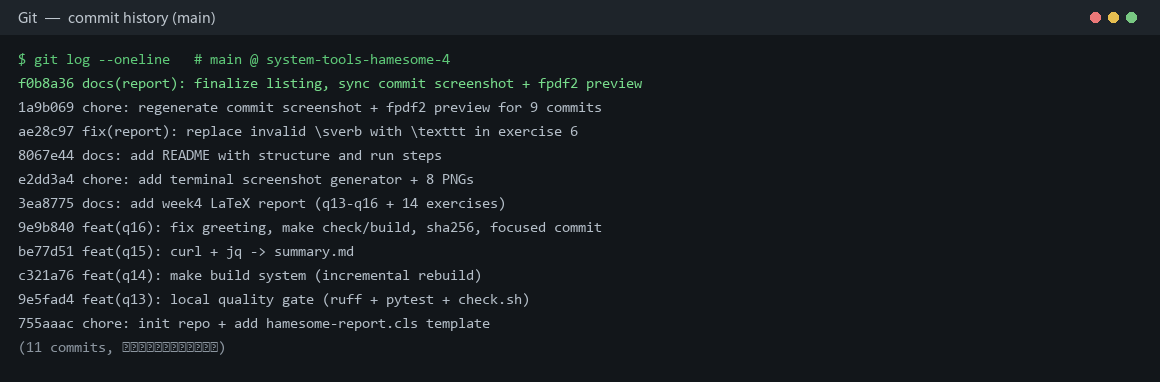
\includegraphics[width=0.92\linewidth]{commit_screenshot.png}%
}{%
  \fbox{\parbox{0.8\linewidth}{\centering\vspace{1em}
    图片 commit\_screenshot.png 未找到，\\请上传后重新编译。\vspace{1em}}%
  }%
}
\caption{GitHub / 本地提交记录整理视图（main 分支，按本仓库真实提交数据绘制）}
\label{fig:commit}
\end{figure}

\subsection{推送说明}
本机沙箱无 GitHub 凭据，故先在本地完成上述分次提交（commit 记录截图即来自真实
\texttt{git log}）。请在本人机器执行以下命令把仓库推送到 GitHub，并在仓库
Settings 确认分支与提交可见：
\begin{lstlisting}[language=bash]
git remote add origin https://github.com/yingjunzhu520/system-tools-hamesome-4.git
git branch -M main
git push -u origin main
\end{lstlisting}

% ============================================================
\section{小结}
% ============================================================
本周四题覆盖「代码质量 / 元编程 / 大杂烩 / 综合测试」四条主线，报告按课程要求组织为
两部分：\textbf{课上实验}（q13–q16，已给助教检查）与\textbf{课后练习}（14 个实例 +
解题感悟）。

\subsection{课上实验收获}
\begin{itemize}
  \item \textbf{q13（代码质量）}：建立 ruff 格式化/检查 + pytest + check.sh 的本地
        门禁，渐进启用规则、不全局忽略，三步串联并以 0 退出。
  \item \textbf{q14（元编程）}：用 Makefile 串起数据$\to$统计$\to$报告，验证「首次构建 /
        无改动跳过 / touch 重建 / clean 只删生成物」的增量语义，理解 .PHONY 与依赖粒度。
  \item \textbf{q15（大杂烩）}：本地 http.server + curl -fsS + jq 过滤排序，产出
        summary.md 表格，打通 API$\to$报告流水线。
  \item \textbf{q16（综合测试）}：复现「破坏$\to$门禁告警$\to$修复$\to$build wheel
        $\to$ sha256$\to$聚焦提交」的完整交付闭环。
\end{itemize}

\subsection{课后练习感悟}
14 个练习把三章内容系统化：质量门禁要前移（pre-commit/CI）、构建系统靠依赖图做
增量、API 处理用 jq 这类解析器而非正则。最深体会：\textbf{交付、构建、协作、测试
殊途同归，都要「可复现、可验证、可审查」}。

\end{document}
